\chapter{AnemoI – AI-Based Weather Modeling}

%==============================================================================
%
%==============================================================================
\section{Yaml and Hydra}

Before we explore AnemoI let us complete our preparation by looking at two main tools used. 

%------------------------------------------------------------------------------
%
%------------------------------------------------------------------------------
\subsection{YAML – Configuration Made Simple}

YAML (YAML Ain't Markup Language) is a human-readable format used for configuration files. It is built on indentation and simple key-value structures, making it ideal for defining settings in machine learning workflows.

In the context of Anemoi and many other ML frameworks, YAML is used to define model parameters, training hyperparameters, and paths. Here's a simple YAML file that defines both a model and a training configuration:

\begin{codeonly}{Model and Training Configuration}
model:
  name: simple_model
  input_size: 10
  hidden_size: 20
  output_size: 1

training:
  epochs: 5
  batch_size: 32
  learning_rate: 0.01
\end{codeonly}

This configuration can be loaded in Python using the \texttt{PyYAML} library and interpreted as a dictionary. Here's an example of how to load it:

\begin{codeonly}{Python: Load YAML}
import yaml

with open("simple_config.yaml", "r") as file:
    config = yaml.safe_load(file)

print("Model name:", config["model"]["name"])
print("Training for", config["training"]["epochs"], "epochs")
\end{codeonly}

You can then pass this configuration into a training function or class:

\begin{codeonly}{Python: Use Configuration}
def train_model(config):
    print(f"Training model '{config['model']['name']}'")
    print("Hyperparameters:")
    print("  Learning rate:", config["training"]["learning_rate"])
    print("  Batch size:", config["training"]["batch_size"])
    for epoch in range(config["training"]["epochs"]):
        print(f"Epoch {epoch+1}... (training logic here)")

train_model(config)
\end{codeonly}

This illustrates how YAML is used as an external, editable source of parameters for training code, enabling experiment reproducibility and flexible configuration.

%------------------------------------------------------------------------------
%
%------------------------------------------------------------------------------
\subsection{Hydra – Flexible Configuration for ML Experiments}

Hydra is a Python framework for managing complex configuration workflows. It allows users to compose and override YAML configuration files at runtime, enabling modular and reusable setups for machine learning experiments. In our example, we train a neural network to learn the function \( y = \sin(x) \), and use Hydra to flexibly switch between different model architectures and training parameters.

\begin{figure}[ht]
  \centering
  \begin{minipage}{0.48\textwidth}
    \centering
    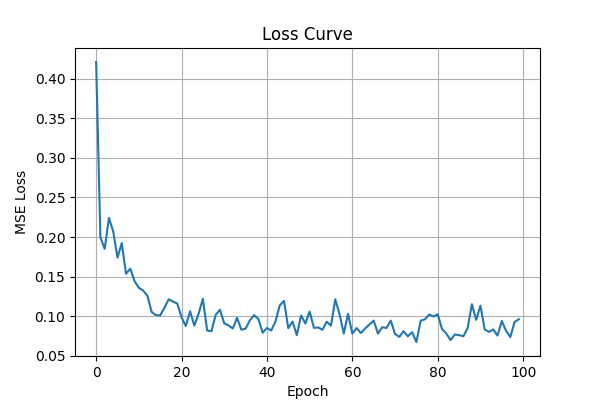
\includegraphics[width=\linewidth]{images/hydra1_mlp.png}
    \caption*{{\bf (a)} Loss curve for the shallow model (\texttt{mlp}). Training converges quickly to a low loss.}
  \end{minipage}
  \hfill
  \begin{minipage}{0.48\textwidth}
    \centering
    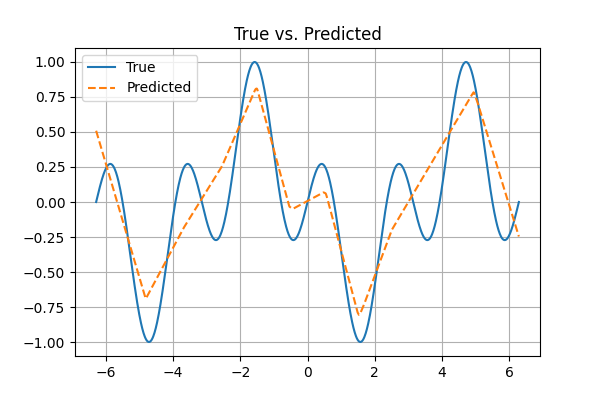
\includegraphics[width=\linewidth]{images/hydra2_mlp.png}
    \caption*{{\bf (b)} Prediction result for the shallow model. The curve closely matches the true $\sin(x)$ target.}
  \end{minipage}

  \vspace{1em}

  \begin{minipage}{0.48\textwidth}
    \centering
    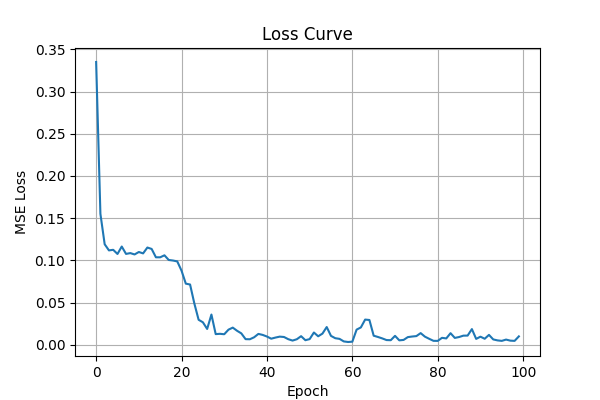
\includegraphics[width=\linewidth]{images/hydra1_deep.png}
    \caption*{{\bf (c)} Loss curve for the deeper model (\texttt{deep}). Training is slower and convergence less stable.}
  \end{minipage}
  \hfill
  \begin{minipage}{0.48\textwidth}
    \centering
    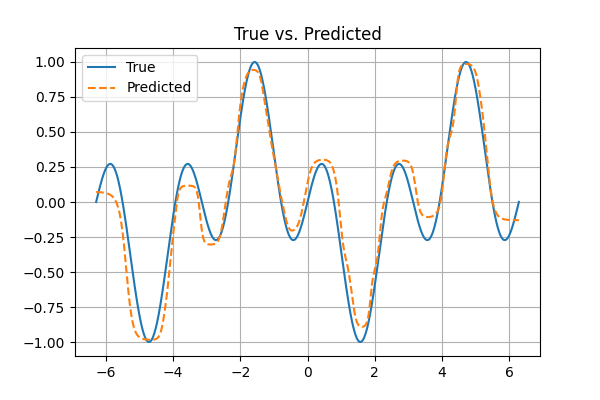
\includegraphics[width=\linewidth]{images/hydra2_deep.png}
    \caption*{{\bf (d)} Prediction result for the deeper model. The curve is less smooth and overshoots the target in places.}
  \end{minipage}

  \caption{Training results for two model configurations defined using Hydra. The shallow model (\texttt{mlp}) performs more effectively for approximating the simple $\sin(x)$ function, while the deeper model (\texttt{deep}) shows signs of overfitting or instability.}
  \label{fig:hydra-mlp-comparison}
\end{figure}


{\bf Base Configuration:} The central Hydra entry point is \texttt{config.yaml}, which specifies which model and training configuration to load:

\begin{codeonly}{config.yaml}
defaults:
  - model: mlp
  - training: simple
  - _self_
\end{codeonly}

{\bf Shallow MLP Configuration:} A simple neural network with one hidden layer is defined like this:

\begin{codeonly}{model/mlp.yaml}
layer_sizes: [1, 64, 1]
activation: relu
\end{codeonly}

{\bf Deeper Network Configuration:} A deeper network with three hidden layers can be defined similarly:

\begin{codeonly}{model/deep.yaml}
layer_sizes: [1, 128, 64, 32, 1]
activation: tanh
\end{codeonly}

{\bf Training Configuration:} Training hyperparameters such as learning rate and batch size are defined in a separate file:

\begin{codeonly}{training/simple.yaml}
epochs: 100
lr: 0.01
batch_size: 32
\end{codeonly}

{\bf Using Hydra in Python:} Hydra supports programmatic configuration loading and overrides using the \texttt{initialize} and \texttt{compose} functions. This allows the configuration to be composed dynamically at runtime, for example to switch between different models within the same training loop.

In the following example, the \texttt{run\_with\_override} function dynamically loads a specified model configuration (e.g., \texttt{mlp} or \texttt{deep}) and then trains the model accordingly.

\begin{codeonly}{Python}
from hydra import initialize, compose

def run_with_override(model_name, title):
    with initialize(config_path="conf", version_base=None):
        cfg = compose(config_name="config", overrides=[f"model={model_name}"])
    print(f"\\n{'='*30}\\nTraining model: {model_name.upper()} ({title})\\n{'='*30}")
    train_model(cfg)

# Run shallow model
run_with_override("mlp", "Shallow Network (1 hidden layer)")
\end{codeonly}

This function uses the Hydra override mechanism:
\begin{codeonly}{Python}
cfg = compose(config_name="config", overrides=[f"model={model_name}"])
\end{codeonly}
to replace the model defined in \texttt{config.yaml} at runtime. For example, if \texttt{model=deep} is used as an override, then \texttt{conf/model/deep.yaml} is loaded instead of the default \texttt{mlp.yaml}.

To demonstrate this in practice, the following snippet dynamically creates a deeper model configuration file (if not already present) and then runs training with it:

\begin{codeonly}{Python}
# Create deep model config if not already created
import os
if not os.path.exists("conf/model/deep.yaml"):
    with open("conf/model/deep.yaml", "w") as f:
        f.write(\"\"\"
layer_sizes: [1, 128, 64, 32, 1]
activation: tanh
\"\"\")

# Run deeper model
run_with_override("deep", "Deeper Network (3 hidden layers)")
\end{codeonly}

This dynamic Hydra setup makes it easy to test and compare different model architectures or training configurations without modifying the underlying training code. It supports flexible experimentation and reproducibility, which is particularly important in complex machine learning pipelines like Anemoi.

%------------------------------------------------------------------------------
%
%------------------------------------------------------------------------------
\subsection{OmegaConf Integration}

Internally, Anemoi relies on \texttt{OmegaConf} to represent and manipulate the hierarchical configuration tree provided by Hydra. Configuration classes like \texttt{BaseSchema} are converted to and from \texttt{DictConfig} objects using OmegaConf utilities.

\begin{itemize}
  \item \textbf{Library:} \url{https://omegaconf.readthedocs.io/}
  \item \texttt{OmegaConf.to\_object(...)} is used to convert validated configs into native Python dictionaries.
  \item \texttt{OmegaConf.resolve(...)} ensures that interpolations and references are evaluated before use.
\end{itemize}

This layer of indirection allows for robust and modular configuration parsing, while still enabling dynamic instantiation via Hydra.

%==============================================================================
%
%==============================================================================
\section{Introduction to AnemoI}

The Anemoi framework, developed by ECMWF and its partners, provides a modular and extensible system for training machine learning models in the context of numerical weather prediction and Earth system modelling. It is designed to facilitate the development, training, and deployment of advanced machine learning architectures tailored to meteorological data, with a focus on scalability, flexibility, and reproducibility. 

The framework is organized into several core packages—responsible respectively for training loops, model definitions, data pipelines, and graph structures—that are now unified under a single repository: \url{https://github.com/ecmwf/anemoi-core}. This monorepo supersedes earlier standalone repositories (such as \texttt{anemoi-training} and \texttt{anemoi-models}), bringing all essential components together for coherent development and integration. This section outlines a structured approach for exploring and understanding the most important elements of the Anemoi codebase, including how data are loaded and preprocessed, how models are constructed, and how training is orchestrated using customizable strategies.

We need to formulate a warning: the anemoi repo has undergoon frequent changes, our links might point to versions which have changed!

%------------------------------------------------------------------------------
%
%------------------------------------------------------------------------------
\subsection{Training Loop}

The training loop orchestrates the entire model training process. It is implemented within the \texttt{anemoi-training} package and uses PyTorch Lightning as its backend. The main entry point is the \texttt{train.py} script, which instantiates an \texttt{AnemoiTrainer} class. This class is responsible for loading configurations, initializing the model and data module, setting up logging and diagnostics, and executing the training via Lightning's \texttt{Trainer.fit()} call.

\begin{itemize}
  \item \textbf{Documentation:} \url{https://anemoi.readthedocs.io/projects/training/en/latest/}
  \item \textbf{Main script:} \href{https://github.com/ecmwf/anemoi-core/blob/main/training/src/anemoi/training/train/train.py}{\texttt{train.py}} (in \texttt{anemoi-core})
  \item \textbf{Configuration:} Training is driven by YAML files parsed via Hydra and OmegaConf. Example configurations can be found in the directory:
  \begin{itemize}
    \item \href{https://github.com/ecmwf/anemoi-core/tree/main/training/src/anemoi/training/config}{\texttt{training/config}} (YAML configs for models, datasets, strategies, etc.)
  \end{itemize}
  \item \textbf{Key modules:}
  \begin{itemize}
    \item \href{https://github.com/ecmwf/anemoi-core/blob/main/training/src/anemoi/training/distributed/strategy.py}{\texttt{strategy.py}} – contains custom distributed training strategies.
    \item \href{https://github.com/ecmwf/anemoi-core/blob/main/training/src/anemoi/training/losses/losses.py}{\texttt{losses.py}} – defines loss functions used during training.
  \end{itemize}
\end{itemize}

When the \texttt{train.py} script is run, it loads a Hydra configuration, builds a model and data pipeline based on the selected YAML files, and begins training with the configured strategy. The modularity of the setup allows the user to customize all elements—data preprocessing, model architecture, logging, and training loop—by simply editing the YAML configuration.

%------------------------------------------------------------------------------
%
%------------------------------------------------------------------------------
\subsection{Model Definitions}

Model architectures and components are implemented in the \texttt{anemoi-models} package, which provides a flexible and modular system to define, compose, and interface neural networks for weather forecasting applications.

\begin{itemize}
  \item {\bf Documentation:} \url{https://anemoi.readthedocs.io/projects/models/en/latest/}
  \item {\bf Source Code:} \url{https://github.com/ecmwf/anemoi-core/tree/main/models/src/anemoi/models}
\end{itemize}

The package is organized into several key modules:

\begin{itemize}
  \item {\bf \texttt{models}:} Implements various network architectures used in Anemoi, such as MLPs, U-Nets, and Graph Neural Networks.\\
  GitHub: \url{https://github.com/ecmwf/anemoi-core/tree/main/models/src/anemoi/models/models}
  
  \item {\bf \texttt{layers}:} Contains reusable components like attention mechanisms, residual blocks, and normalization layers that can be used across models.\\
  GitHub: \url{https://github.com/ecmwf/anemoi-core/tree/main/models/src/anemoi/models/layers}
  
  \item {\bf \texttt{interface}:} Defines the standard model interface used for integration into the Anemoi training loop. Models inherit from LightningModule and conform to standardized input/output conventions.\\
  GitHub: \url{https://github.com/ecmwf/anemoi-core/tree/main/models/src/anemoi/models/interface}
\end{itemize}

These modules are configured and instantiated dynamically using Hydra, allowing flexible model selection and hyperparameter tuning via YAML configuration files.

%------------------------------------------------------------------------------
%
%------------------------------------------------------------------------------
\subsection{Data Handling}

The data loading and preprocessing logic is described in the \texttt{anemoi-datasets} documentation, which outlines how structured and graph-based meteorological datasets are processed. While the public source code for this package is not currently available, the interfaces are fully described and configurable via YAML and Hydra.

\begin{itemize}
  \item {\bf Documentation:} \url{https://anemoi.readthedocs.io/projects/datasets/en/latest/}
\end{itemize}

Key components (as documented) include:

\begin{itemize}
  \item {\bf \texttt{datasets}:} For loading structured or graph-ready datasets from formats like GRIB or NetCDF.
  \item {\bf \texttt{preprocessing}:} For transformations such as normalization, filtering, and feature generation.
\end{itemize}

Users define data behavior declaratively via YAML configuration files. These definitions are passed to the training and graph modules via Hydra, ensuring reproducibility and modularity across workflows.


%------------------------------------------------------------------------------
%
%------------------------------------------------------------------------------
\subsection{Graph Structures}

Graphs are used in Anemoi to represent spatial and temporal dependencies in meteorological data. These graph-based structures enable Graph Neural Networks (GNNs) to model interactions between grid cells or observation points effectively. The \texttt{anemoi-graphs} package provides tools for generating and managing these graph representations.

\begin{itemize}
  \item {\bf Documentation:} \url{https://anemoi.readthedocs.io/projects/graphs/en/latest/}
  \item {\bf Source Code:} \url{https://github.com/ecmwf/anemoi-core/tree/main/graphs/src/anemoi/graphs}
\end{itemize}

Key components include:

\begin{itemize}
  \item {\bf \texttt{graphs}:} Provides utilities to construct and serialize graphs from model grids, using distance-based, nearest-neighbor, or mesh-specific methods (e.g., for ICON or IFS grids).\\
  GitHub: \url{https://github.com/ecmwf/anemoi-core/tree/main/graphs/src/anemoi/graphs}
  
  \item {\bf Integration with Models:} Graph objects are generated once and passed to the model and datamodule. This allows for consistent and reusable topology definitions across experiments. Graph data can be saved as PyTorch tensors and reloaded at runtime.
\end{itemize}

Graph definitions are fully configurable via Hydra YAML files. Users can specify graph types, node layouts, edge construction logic, and file paths, making the process flexible and reproducible across model setups.


%==============================================================================
%
%==============================================================================
\section{Training Pipeline in Anemoi}

The training process in Anemoi is managed by the script \texttt{train.py} in the \texttt{anemoi-training} package. It implements a highly modular, Hydra-driven architecture built on top of PyTorch Lightning. The main orchestration is encapsulated in the \texttt{AnemoiTrainer} class, which configures, initializes, and runs model training and evaluation.

%------------------------------------------------------------------------------
%
%------------------------------------------------------------------------------
\subsection{Hydra Entry Point and Configuration}

The training is launched via a Hydra-decorated function at the end of \texttt{train.py}:

\begin{codeonly}{Hydra Entry Point}
@hydra.main(version_base=None, config_path="../config", config_name="config")
def main(config: DictConfig) -> None:
    AnemoiTrainer(config).train()
\end{codeonly}

This function is the command-line entry point to Anemoi training jobs. Hydra parses the YAML configuration files into a nested \texttt{DictConfig} object and injects it into the trainer.

The configuration system supports:
\begin{itemize}
  \item Model and data module selection
  \item Training hyperparameters
  \item Graph and truncation settings
  \item Logging, callbacks, and checkpointing
\end{itemize}

{\bf Source code:} \url{https://github.com/ecmwf/anemoi-core/blob/main/training/src/anemoi/training/train/train.py}

%------------------------------------------------------------------------------
%
%------------------------------------------------------------------------------
\subsection{AnemoiTrainer Class Overview}

The \texttt{AnemoiTrainer} class is the core wrapper for the entire experiment lifecycle. It performs:

\begin{itemize}
  \item Validation and conversion of the Hydra configuration schema
  \item Setup of metadata, seeds, run IDs, and logging paths
  \item Construction or loading of graph and truncation data
  \item Initialization of the data module and model via Hydra
  \item Creation of callbacks and loggers (MLflow, TensorBoard, W\&B)
\end{itemize}

Many of these components are defined as \texttt{@cached\_property}, ensuring lazy and consistent instantiation. For instance:

\begin{codeonly}{Core Cached Properties}
@property
def datamodule(self) -> Any: ...
@property
def graph_data(self) -> HeteroData: ...
@property
def model(self) -> pl.LightningModule: ...
\end{codeonly}

{\bf AnemoiTrainer class:} \url{https://github.com/ecmwf/anemoi-core/blob/main/training/src/anemoi/training/train/train.py#L58}

%------------------------------------------------------------------------------
%
%------------------------------------------------------------------------------
\subsection{Model and Data Instantiation}

The model and data modules are instantiated dynamically from the YAML config using Hydra utilities:

\begin{codeonly}{Dynamic Instantiation}
model_task = get_class(self.config.training.model_task)
model = model_task(
    config=self.config,
    data_indices=self.data_indices,
    graph_data=self.graph_data,
    ...
)

datamodule = instantiate(
    convert_to_omegaconf(self.config).datamodule,
    convert_to_omegaconf(self.config),
    self.graph_data,
)
\end{codeonly}

This allows complete flexibility: different models and datasets can be specified per experiment without code changes.

%------------------------------------------------------------------------------
%
%------------------------------------------------------------------------------
\subsection{Training Execution via Lightning}

The actual training is launched by calling the \texttt{train()} method of the trainer, which constructs a \texttt{pl.Trainer} instance and calls \texttt{fit()}:

\begin{codeonly}{Lightning Training Loop}
trainer = pl.Trainer(
    accelerator=self.accelerator,
    callbacks=self.callbacks,
    strategy=self.strategy,
    logger=self.loggers,
    max_epochs=self.config.training.max_epochs,
    ...
)
trainer.fit(
    self.model,
    datamodule=self.datamodule,
    ckpt_path=None if self.load_weights_only else self.last_checkpoint,
)
\end{codeonly}

PyTorch Lightning handles the boilerplate of device placement, training/validation looping, and checkpointing. Logging is automatically integrated with MLflow or Weights \& Biases depending on the configuration.

{\bf Training execution (\texttt{trainer.fit}):} \url{https://github.com/ecmwf/anemoi-core/blob/main/training/src/anemoi/training/train/train.py#L509}


%------------------------------------------------------------------------------
%
%------------------------------------------------------------------------------
\subsection{Configuration and Schema Management}

Anemoi uses configuration schemas defined in \texttt{schemas/base\_schema.py} to validate and standardize the structure of the configuration:

\begin{itemize}
  \item \texttt{BaseSchema} is the validated config interface.
  \item \texttt{UnvalidatedBaseSchema} is used for lenient mode.
  \item Conversion utilities ensure compatibility with OmegaConf and Hydra.
\end{itemize}

This system guarantees consistency across model runs and supports reproducibility by recording full config metadata.

{\bf Config Schema:} \url{https://github.com/ecmwf/anemoi-core/blob/main/training/src/anemoi/training/schemas/base_schema.py}


%------------------------------------------------------------------------------
%
%------------------------------------------------------------------------------
\subsection{Graph and Truncation Handling}

Graph and truncation matrices are prepared before model initialization. If precomputed files exist, they are loaded; otherwise, they are created:

\begin{codeonly}{Graph Creation}
from anemoi.graphs.create import GraphCreator
graph = GraphCreator(config=graph_config).create(...)
\end{codeonly}

Truncation matrices (used for resolution conversion) are loaded via SciPy sparse utilities and passed to the model.

%------------------------------------------------------------------------------
%
%------------------------------------------------------------------------------
\subsection{Summary}

The Anemoi training pipeline brings together Hydra for flexible configuration, PyTorch Lightning for robust training infrastructure, and ECMWF-specific data tools for handling graph and weather model inputs. The \texttt{AnemoiTrainer} class encapsulates the orchestration of these components, making experiments declarative, reproducible, and modular.


%==============================================================================
%
%==============================================================================
\section{Core Architecture and AI Components}
AnemoI leverages a combination of neural networks and physics-informed machine learning to model atmospheric processes. The system integrates with conventional forecasting models to improve accuracy and computational efficiency.

%==============================================================================
%
%==============================================================================
\section{Training AnemoI with Historical Weather Data}
To develop robust AI models, AnemoI is trained on large-scale reanalysis datasets, satellite observations, and in-situ measurements. This section outlines the preprocessing, feature selection, and data augmentation techniques used for training.



